\begin{ledgroupsized}[r]{120mm}
\footnotesize
\pstart
\noindent\textbf{\"{U}berlieferung:}
\pend
\end{ledgroupsized}
\begin{ledgroupsized}[r]{114mm}
\footnotesize
\pstart
\parindent -6mm
\makebox[6mm][l]{\textit{L}}Konzept: LH XXXVII 5 Bl. 12. 1 Bl. 4\textsuperscript{o}. Etwas weniger als 1 \nicefrac{1}{2} S. Das St\"{u}ck N. 31\textsubscript{2} schlie{\ss}t unmittelbar an N. 31\textsubscript{1} an. In der Mitte von Bl. 12~v\textsuperscript{o} beginnt Nr. 31\textsubscript{3}. \"{U}berschrift und Datierung nachtr\"{a}glich hinzugef\"{u}gt. \\Cc 2, Nr. 945 B
\pend
\end{ledgroupsized}
\vspace*{8mm} 
\pstart
\noindent
[12~r\textsuperscript{o}] \edtext{April 1675}{\lemma{}\Bfootnote{April 1675 \textit{erg.} \textit{L}}}
\pend
\count\Afootins=1200
\count\Bfootins=1200
\count\Cfootins=1200
\vspace*{1em}
\pstart
\centering
\edtext{\textso{De Detrimento Motus.} Frottement}%
{\lemma{\textso{De Detrimento Motus.} Frottement}\Bfootnote{\textit{erg. L}}}
\pend 
\pstart \vspace*{0.5em} \noindent
Ut consideretur retardatio a resistentia medii\protect\index{Sachverzeichnis}{resistentia medii} ponatur pila $A$ labi \edtext{motu uniformi}{\lemma{}\Bfootnote{motu uniformi \textit{erg.} \textit{L}}}, et obstacula superanda reperire $B$, $D$, $E$. Ponenda autem sunt obstacula virium\protect\index{Sachverzeichnis}{vis} aequalium. Jam majori celeritati\protect\index{Sachverzeichnis}{celeritas} magis etiam obsistit \edtext{obstaculum.\\
\hspace*{7,5mm}
Motus}{\lemma{obstaculum.}\Bfootnote{\textit{(1)}\ Conatus \textit{(2)}\ Motus \textit{L}}} 
ipsius $A$, sit $m$, fiet vis ejus $Am$. Resistentia ipsius $B$ sit $r$, et tota resistentia erit $Br$. Ponatur aliquod pondus\protect\index{Sachverzeichnis}{pondus} esse elevandum a motione obstaculi. Quod pondus ad ipsum pondus $A$, habeat rationem $\rule[-4mm]{0mm}{10mm} \displaystyle \frac{b}{r}$, et erit $\rule[-4mm]{0mm}{10mm} \displaystyle 
\edtext{\frac{b}{r}A$. Celeritas}{\lemma{$\displaystyle\frac{b}{r}A$.}\Bfootnote{\textit{(1)}\ Motus \textit{(2)}\ Celeritas \textit{L}}}
ipsius $A$, sit $C$, erit vis ejus $CA$. Ergo resistentia ipsius $B$ erit $ \displaystyle \frac{b}{r}\,CA$. 
\edtext{Ergo si}{\lemma{Ergo}\Bfootnote{\textit{(1)}\ vel a \textit{(2)}\ si \textit{L}}} per minimum tantum spatium fingamus
\pageparbreak
attolli pondus \edtext{ita ut nulla habenda sit spatii ratio}{\lemma{}\Bfootnote{ita [...] ratio \textit{erg.} \textit{L}}}, erit vis ipsius $A$, post impulsum\protect\index{Sachverzeichnis}{impulsus} $\rule[-4mm]{0mm}{10mm} \displaystyle \edtext{CA,\smallfrown 1- \frac{b}{r}$.\\
\hspace*{7,5mm}
Secunda autem resistentia}{\lemma{$\displaystyle CA,\smallfrown 1- \frac{b}{r}$}\Bfootnote{\textit{(1)}\ et post secundum obstaculum superatum, erit $\displaystyle CA,\smallfrown 2- \frac{2b}{r}$ et post tertium superatum $\displaystyle CA,\smallfrown 3- \frac{3b}{r}$ vel pro 1. 2. 3. ponendo $\displaystyle \frac{y}{r}$, fiet post quodcunque obstaculum superatum, vis residua: $\displaystyle CA,\smallfrown ry-\frac{yb}{r^2}$ \textit{(2)}\ . Secunda autem resistentia \textit{L}}}
est non amplius $\displaystyle \frac{b}{r}\,CA$, sed $\displaystyle \frac{b}{r}A$, obstaculum ductum in 
     celeritatem residuam $\rule[-4mm]{0mm}{10mm} \displaystyle C,\smallfrown 1-\frac{b}{r}$ seu: $\rule[-4mm]{0mm}{10mm} \displaystyle \frac{b}{r}-\frac{b^2}{r^2},\smallfrown CA$.
\edtext{}{\lemma{}\Afootnote{\textit{Am Rand, schräg  und gestrichen:} Nimirum quantitate aliqua data secunda\textsuperscript{[a]} $\displaystyle 1 - \frac{b}{r}$. sequens ita fiet: quaelibet quantitas ducta in $\displaystyle \frac{b}{r}$ subtrahatur a se ipsa.
\\ % PR: Marginalienapparat.
\footnotesize
\textsuperscript{[a]} secunda\ \textit{(1)}\ $\displaystyle \frac{b}{r}$\ \textit{(2)}\ $\displaystyle 1 - \frac{b}{r}$.\ \textit{(a)}\ reliquae ita fient:\ \textit{(b)}\ sequens ita fiet: \textit{L}\vspace{-6mm}}}
\pend 
\pstart
\begin{wrapfigure}[9]{l}{0.17\textwidth}   
\vspace{-3mm}                 
    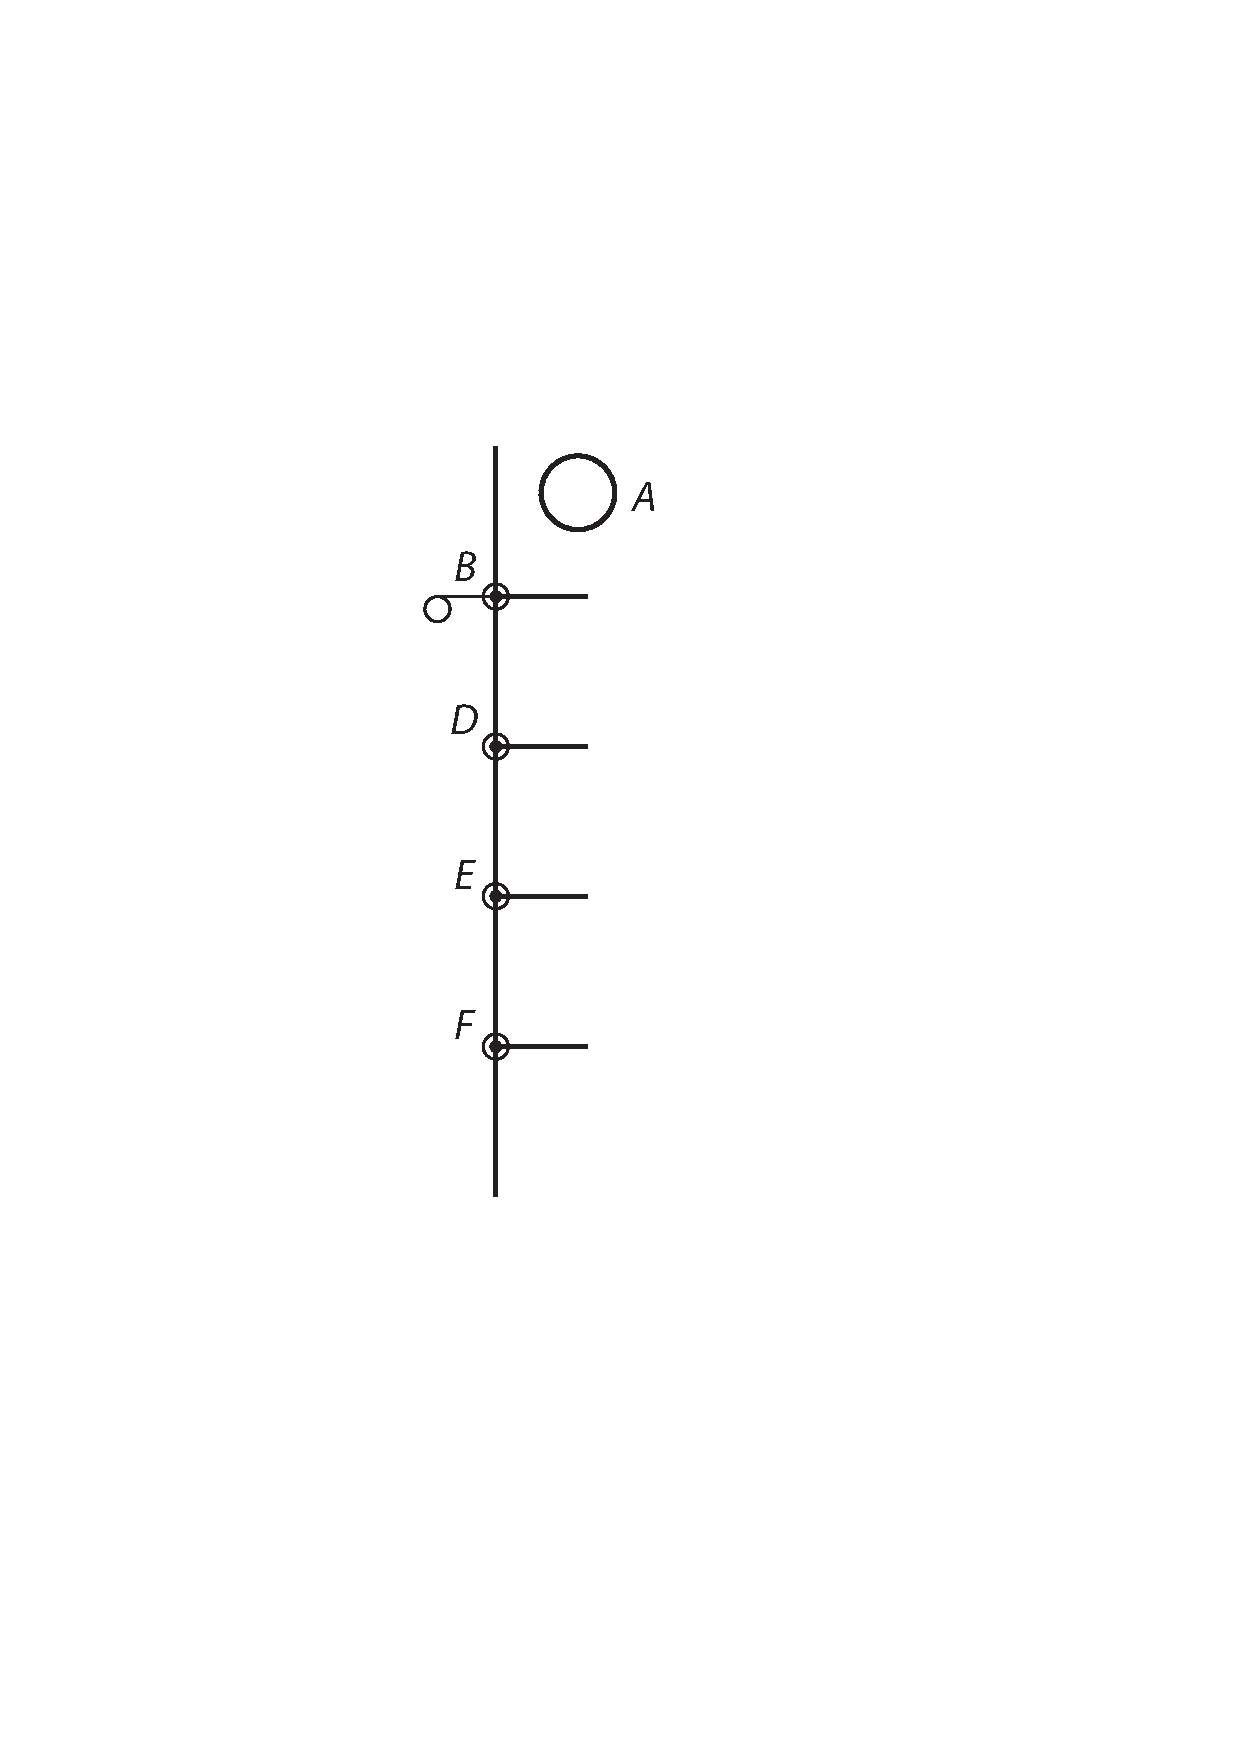
\includegraphics[trim = 0mm -1mm -5mm 0mm, clip, width=0.16\textwidth]{images/lh03705_012r_2-d1.pdf} 
     \noindent \centering [\textit{Fig. 1}]  % \caption{Bildbeschreibung}
     \end{wrapfigure}
$\displaystyle$
Adeoque post hoc obstaculum quoque superatum residua ipsius $A$ celeritas est: $\rule[-4mm]{0mm}{10mm} \displaystyle 1 - \frac{2b}{r} + \frac{b^2}{r^2},\smallfrown C$ quae rursus ductu in $\rule[-4mm]{0mm}{10mm} \displaystyle \frac{b}{r} A$, dabit tertiam Resistentiam: $\rule[-4mm]{0mm}{10mm} \displaystyle CA,\smallfrown \frac{b}{r}-\frac{2b^2}{r^2}+\frac{b^3}{r^3}$.
\\
\hspace*{7.5mm}
%\pend
%\pstart
$\displaystyle$Adeoque post hoc quoque superatum obstaculum residua ipsius $A$ celeritas est: $\rule[-4mm]{0mm}{10mm} \displaystyle 1-\frac{3b}{r}+\frac{3b^2}{r^2}-\frac{b^3}{r^3},\!,\smallfrown C$ quae rursus ductu in $\rule[-4mm]{0mm}{10mm} \displaystyle \frac{b}{r}A$, dabit quartam resistentiam: $\rule[-4mm]{0mm}{10mm} \displaystyle CA, \smallfrown \rule[-4mm]{0mm}{10mm} \displaystyle \frac{b}{r} - \frac{3b^2}{r^2} + \frac{3b^3}{r^3} - \frac{b^4}{r^4}$.\\
\hspace*{7.5mm}
$\displaystyle$Adeoque post hoc quoque superatum obstaculum residua ipsius $A$ celeritas erit: $\rule[-4mm]{0mm}{10mm}\displaystyle 1 - \frac{4b}{r} + \frac{6b^2}{r^2} - \frac{4b^3}{r^3} + \frac{b^4}{r^4}$. Nec opus est ultra progredi, satis enim apparet ratio progressionis.
\pend
%\newpage
\count\Afootins=1200
\count\Bfootins=1200
\count\Cfootins=1200
\pstart
Nimirum si vis quaedam uniformi celeritate progrediatur nisi quatenus celeritas ejus obstaculo objecto diminuitur \edtext{qualis esset motus projectorum, nulla ponderatione gravitatis\protect\index{Sachverzeichnis}{gravitas}, ut in plano horizontali}{\lemma{}\Bfootnote{qualis [...] horizontali \textit{erg.} \textit{L}}}; et obstaculum quoque sit \edtext{uniforme sive semper aequale: nec}{\lemma{uniforme}\Bfootnote{\textit{(1)}\ : nec \textit{(2)}\  et obstaculum \textit{(3)}\  sive semper aequale: nec \textit{L}}} \edtext{dimovendum, nisi}{\lemma{nec}\Bfootnote{\textit{(1)}\ nisi \textit{(2)}\ dimovendum, nisi \textit{L}}} per spatium infinite parvum, quemadmodum si corpus projectum gravitate carens per medium \edtext{perfecte }{\lemma{}\Bfootnote{perfecte  \textbar\ liquidum, sive \textit{gestr.}\ \textbar\ homogeneum \textit{L}}}homogeneum, tenacitate quadam praeditum ferri intelligatur. 
Tunc vi ipsa posita ut 1. et obstaculo ut $\rule[-4mm]{0mm}{10mm} \displaystyle \frac{b}{r}$, erit \edtext{primo loco vis}{\lemma{primo}\Bfootnote{\textit{(1)} momento vis \textit{(2)}   \textbar\ momento \textit{streicht Hrsg.} \textbar\  loco vis \textit{L}\hspace{-2mm}}} ut 1, secundo loco ut $\rule[-4mm]{0mm}{10mm} \displaystyle 1 - \frac{b}{r}$. \edtext{latus}{\lemma{}\Bfootnote{latus \textit{erg.} \textit{L}\hspace{-2mm}}}[;] tertio ut \edtext{quadratum}{\lemma{}\Bfootnote{qua\-dratum \textit{erg.} \textit{L}}} $\rule[-4mm]{0mm}{10mm} \displaystyle 1-\frac{2b}{r}+\frac{b^2}{r^2}$; quarto ut \edtext{cubus}{\lemma{}\Bfootnote{cubus \textit{erg.} \textit{L}}} $\rule[-4mm]{0mm}{10mm} \displaystyle 1-\frac{3b}{r}+\frac{3b^2}{r^2}-\frac{b^3}{r^3}$, quinto \edtext{quadrato-quadratum}{\lemma{}\Bfootnote{quadrato-quadratum \textit{erg.} \textit{L}}} $\rule[-4mm]{0mm}{10mm} \displaystyle 1 - \frac{4b}{r} + \frac{6b^2}{r^2} - \frac{4b^3}{r^3} + \frac{b^4}{r^4}$ et ita porro. Id \edtext{est[:] Numerorum}{\lemma{est[:]}\Bfootnote{\textit{(1)}\ Numeri \textit{(2)}\ Numerorum \textit{ L}}} Combinatoriorum series exponantur signis alternatim affirmatis et negatis; et terminis \edtext{progressionis Geometricae}{\lemma{}\Afootnote{\textit{\"{U}ber} progressionis Geometricae: $\bigl($Imo sunt potestates ab $\displaystyle 1 - \frac{b}{r}.\bigr)$ NB\vspace{-6mm}}}, ab unitate incipientibus ratione $\rule[-4mm]{0mm}{10mm}\displaystyle \frac{b}{r}$ continue, unusquisque terminus seriei per eundem ordine terminum progressionis multiplicetur. Quodsi cogitemus praeterea vim ipsius $A$, esse continue acceleratam longe ni fallor implicatior erit inquisitio. Crescent enim vires cum locis \edtext{ut differentiae [applicatarum]\edtext{}{\Bfootnote{applicatae\textit{\ L \"{a}ndert Hrsg.}}}}{\lemma{ut}\Bfootnote{\textit{(1)}\ applicatae \textit{(2)}\ differentiae [applicatarum] \textit{L}}} parabolae ad axem. Eaedem autem decrescent modo dicto. Non dubito arcanam aliquam in his latere calculi harmoniam, sed quam forte eruet posteritas. $\rule[-4mm]{0mm}{10mm}\displaystyle\Bigl(%
\edtext{\sqrt{2ax + a\beta}}{\lemma{$\displaystyle\sqrt{2ax + a\beta}$}\Cfootnote{Der richtige Radikand lautet $\displaystyle 2ax + 2a\beta$. Der Fehler wirkt sich auf den berechneten Wert von $\displaystyle z$ aus. Der richtige Wert ist $\displaystyle z = \beta\sqrt{\frac{a}{2x}}$.}}
%
- \sqrt{\mathstrut 2ax} \ \sqcap \, z$. \ $\protect\rule[-4mm]{0mm}{10mm}\displaystyle\protect\ovalbox{$2ax$} + \beta a \ \sqcap \ \protect\cancel{z^2} + 2z\sqrt{\protect\mathstrut 2ax} \ \, \protect\ovalbox{$+ \, 2ax$}\,$.
%
Unde $\rule[-4mm]{0mm}{10mm} \displaystyle \beta ^2 a \cancel{^2} \, \sqcap \ 8z^2\cancel{a}x$, sive $\protect\rule[-4mm]{0mm}{10mm} \displaystyle z \, \sqcap \, 2 \beta \sqrt{\protect\vphantom{\frac{2a}{x}}}\frac{2a}{x}$.$\Bigr)$%
%$\rule[-4mm]{0mm}{10mm}\displaystyle\Bigl(\sqrt{2ax + a\beta} - \sqrt{\mathstrut 2ax} \ \sqcap \, z$. \ \edtext{$\protect\rule[-4mm]{0mm}{10mm}\displaystyle\protect\ovalbox{$2ax$} + \beta a \ \sqcap \ \protect\cancel{z^2} + 2z\sqrt{\protect\mathstrut 2ax} \ \, \protect\ovalbox{$+ \, 2ax$}\,$.}{\lemma{$\displaystyle\protect\ovalbox{$2ax$} + \beta a \ \sqcap \ \protect\cancel{z^2} + 2z\sqrt{\protect\mathstrut 2ax} \ \, \protect\ovalbox{$+ \, 2ax$}\,$}\Cfootnote{Die Vernachl\"{a}ssigung von $\displaystyle z^2$ ist unzul\"{a}ssig.}}
%Unde $\rule[-4mm]{0mm}{10mm} \displaystyle \beta ^2 a \cancel{^2} \, \sqcap \ 8z^2\cancel{a}x$, sive \edtext{$\protect\rule[-4mm]{0mm}{10mm} \displaystyle z \, \sqcap \, 2 \beta \sqrt{\protect\vphantom{\frac{2a}{x}}}\frac{2a}{x}$.}{\lemma{$\displaystyle z \, \sqcap \, 2 \beta \sqrt{\protect\vphantom{\frac{2a}{x}}}\frac{2a}{x}$}\Cfootnote{Die Ableitung ist falsch. Richtig heißt es: $\displaystyle z = 2 \beta \sqrt{\frac{2a}{8x}}$.}}$\Bigr)$\!
% \pend
